\chapter{Methods and Materials}
Introduction to chapter




%------------------------------------------------------------------%
\section{Data Collection Hardware}
First hand data

What are the requirements for the sensing system - 100Hz, non-intrusive, simple to operate, can be operated on your own

% Sensor selection and location
% Non-invasive wearable sensors, such~as Inertial Measurement Units (IMU), are~an appealing choice for developing such a system. IMUs~give fast update rates, 100s of Hz, are~non-invasive (small with minimal mounting constraints), low~cost and have reasonable accuracy. They~have been widely used in the field, all~of the latest generation of powered prosthetic knees investigated by Fluit et al contained IMUs~\cite{Fluit2020}.


\subsection{Movesense Sensor}
The platform chosen for data collection is the Suunto Movesense. This is low cost (~£70) Commercial Off The Shelf (COTS) device containing a nine-axis IMU/MARG sensor, heart rate monitor, temperature sensor and a Bluetooth Low Energy (BLE) radio in a small 10g package. The on-board IMUs sensors are factory calibrated so no additional sensor calibration is required. The device is powered by a small coin cell battery that allows for continuous operation for multiple hours. Figure \ref{fig:methods-movesense-sensor} shows a picture of the Movesense device.

\begin{figure}[!hbt]
    \centering
    % \includegraphics{}
    \caption{Movesense Wearable IMU}
    \label{fig:methods-movesense-sensor}
\end{figure}

Custom software can be installed allowing for bespoke setup of the device using the Software Development Kit (SDK) provided by Suunto. In this software device hardware is accessed through calls to the sensor Application Programming Interface (API). A custom program was produced that subscribed to the 100Hz MARG output, heart rate and temperature sensor. These were then transmitted over BLE to a android app for data logging. Further details on these steps are presented in subsequent sections.

The software also implemented power management, placing the sensors in a ultra-low power state when inactive, as detected by the accelerometer, for more than 10 minutes. The devices could then be woken again by pressing the rear contacts. This wake interrupt detection is a feature of the on board heart rate monitoring sensors.

The device's rear contact also act as mounting point for attaching the device to a wide variety of sensors. These include heart rate straps and Velcro strap. Five sensors were attached to each participant in the following locations: on the inside of both ankles using an elastic Velcro strap, on~each hip using a clothes/belt clip and across the chest using a heart rate strap. The location of the sensors was selected to give wide coverage of body movements while providing easy, secure and non-invasive attachment to minimize discomfort and disruption to natural movement. Figure~\ref{fig:methods-movesense-sensor-locations} shows a subject wearing the five sensors.

\begin{figure}[!hbt]
    \centering
    % \includegraphics{}
    \caption{Movesense sensor attachment locations}
    \label{fig:methods-movesense-sensor-locations}
\end{figure}

% How is sensor data transmitted 
\subsubsection{BLE Data Transmission}
\label{subsection:methods-on-sensor-compression}
Data is transmitted wireless using the built in Bluetooth Low Energy (BLE) transceiver in the Movesense to a connected smartphone. The process for preparing the sensor data for transmission is presented below.

A custom GATT service was created that allows data packed to be pushed to a connected smartphone. Data pushing is done using the BLE notify mechanism. Data streaming starts when a notify state is set on the BLE characteristic. It stops again when the notify state is cleared. Only enters the high power draw streaming state when recording.

Two limits restrict the data rate that the sensor can transmit. The maximum individual packet size that can be transmitted by the Movesense device is 155 bytes long. There is also a maximum practical transmission rate of less than 15Hz, due to requirements for transmission concurrently from five sensors. The transmission limit require that to achieve a 100Hz sample rate multiple IMU samples are transmitted per packet.

IMU data from the sensor is provided as a 32-bit floating point number. Each sample of the three axis for each of the three sensors requires 36 bytes. At full size only four samples can be packed within the limit for a single BLE transmission. Therefore compression of the data is required.

Compressing the data to 16-bit fixed point signed integer values allow for eight packets of data to be transmitted concurrently. The compression is achieved by multiplying the original value by a scaling factor before typecast to a int-16. This retains the sub-decimal accuracy while allowing for sufficient compression. Table \ref{tab:methods-imu-data-compression-factors} presents the sensor ranges, scaling factors and resultant accuracy of each sensor. As 16-bit integer values have a maximum range of $-32,768$ to $32,767$ clipping would occur if the scaled value of the sensors exceeds this. The scaling factor was therefore chosen as a balance between accuracy and output range with the output range requirement calculated experimentally.

\begin{table}[!hbt]
    \centering
    \caption{Table of sensor compression factors and resultant accuracy. G --- Force of Gravity, DPS --- Degrees per Second, $\mu T$ --- MicroTesla}
    \label{tab:methods-imu-data-compression-factors}
    
    \begin{tabular}{l|ccc}
         \textbf{Sensor} & \textbf{Sensor Range} & \textbf{Scaling Factor} & \textbf{Accuracy} \\
         \hline
         Acceleromenter & $\pm16 G$ & $256$ & $\pm0.039 G$  \\
         Gyroscope & $\pm2000 DPS$ & $32$ & $\pm0.031 DPS$  \\
         Magnetometer & $\pm5000\mu T$ & $1$ & $\pm1\mu T$
    \end{tabular}
\end{table}

Once compressed 8 IMU samples fit within one packet leaving 11 bytes available. A timestamp based on the internal sensor clock is transmitted as a 32-bit unsigned integer. Six further bytes is populated with the temperature, heart rate and R-R interval recording from the sensor. These were added for future use. As these values are only provided by the sensor on a change in value the remaining byte is used as a update flag for each field. Figure \ref{fig:methods-ble-packet-structure} illustrates the full 155 byte transmission packet.

\begin{figure}[!hbt]
    \centering
    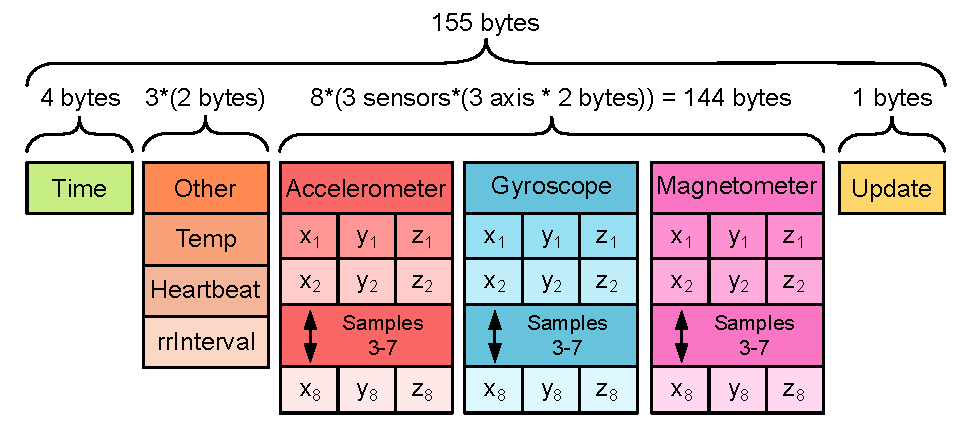
\includegraphics[width=0.9\textwidth]{content/3-Methods/BLE_Bytes_Packets.pdf}
    \caption{Bluetooth Low Energy characteristic transmission packet structure}
    \label{fig:methods-ble-packet-structure}
\end{figure}

\subsection{Android App}
The BLE data stream is received by a smart phone held by the participant. This serves three purposes: to save the sensor data, to annotate the current activity, and to share annotated data with the researcher. These three steps are described in more detail below. 

In recording mode three services run; User Interface (UI) and BLE and file background services. The UI service commands the BLE and File services based on user input and also relays information from the two background services to the user. This information includes errors with the sensors and recording statistics. An illustration of the interactions between each aspect of the app is shown in Figure \ref{fig:methods-android-app}.

\begin{figure}[!hbt]
    \centering
    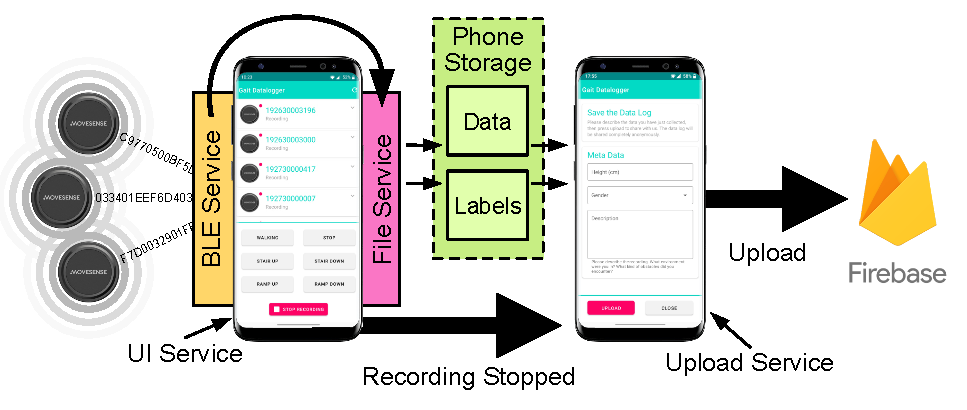
\includegraphics[width=0.9\textwidth]{content/3-Methods/Android_App.pdf}
    \caption{Data-logging Android App}
    \label{fig:methods-android-app}
\end{figure}

\subsubsection{User Interface}
The user interface of the app is intentionally simple requiring minimal instruction to use. The interface is handled by the UI service. A BLE connection is automatically established with any 'on' sensor that is detected during a BLE device scan when the app opens. If not all sensors are found this search can be repeated.

During recording a series of buttons at the bottom of android app are used to annotate the current activities. Each time a button is pressed the file service records both the name of the button and the phone timestamp to a label file.

Once recording had finished the user is presented with an upload screen allowing metadata to be added and data to be shared with researchers.

\subsubsection{Saving Sensor Data}
The android app is primarily responsible for forming a BLE connection to each sensor and saving the sensor data stream to a file that could be interpreted later. This BLE connection is managed by a background BLE service in the app.

Record is started by the subject pressing the record button. The app then sets the notify state on each device starting data streaming. Received data is passed from the BLE service to the file saving service. This service creates plain text files locally on the phone. Each message of data is saved on a new line in the file along with the phone time stamp and MAC address of the sensor. The data message is saved as a hexadecimal representation of the received binary data string. All sensors are saved together in a single file with each line representing a received BLE data message.

The saved file can then be shared anonymously with the researchers using Google's Firebase cloud services. This uploads the files saved to the phone to google's cloud servers for later retrieval by researchers.

\section{Data Collection}
First hand data

Introduction and purpose of data collections

What is unique about our data set
- Unsupervised - Provided with sensors, app and basic instructions of how to setup and label data
- Wide range of different natural environments and terrain
- Large number of people

%Ethics Approval
The~study received ethical approval from the University of Bath Research Ethics Approval Committee for Health (REACH), reference \textit{EP 19/20 003}.

\subsection{Activities}
What activities are we recording. What is the justification for this split

% The following activities were selected, Walking (W), Stair Ascent (SA), Stair Descent (SD), Ramp Ascent (RA), Ramp~Descent (RD) and Stopped (S). Labarri\`ere et al. identified these as the most commonly investigated and they require no equipment or skill to perform~\cite{Labarriere2020}. 

% Pictures showing the variety of terrain %

How were the subjects instructed to label data - press at first HS on new activity

\subsection{Recording Procedure}
% Does this belong here - probably covered by each individual section
% 
% Study subjects were provided with instructions on how to use the sensing equipment, and~the activity classes, then~allowed to record as they wished.

% Twenty-two participants of a wide variety of age (mean 29, std~10), gender (17M, 5F), and~physique were chosen to give a broad data set. Participants were instructed to walk around a varied environment with the sensor on while labelling the six activity classes. No~further instructions on how the recording should be conducted were provided.


\subsection{Data-set Summary} 
% % Participant instructions
 A~total of 268~min  of data was collected, which includes 1170~transitions between activities. Table \ref{tab:data_collected_summary} contains a summary of the data collected. The~number of steps was produced by summing the peak swing gait events for each label.
% Summarise data connected

% Collected in three phases - 
% broad range of people - 22 participants
% TABLE OF DATA SUMMARY %

% Present collected data - table of amounts per participant (How many episodes, stats on episodes)
% TABLE OF DATA SUMMARY % 

% Amputee data
% TABLE OF DATA SUMMARY %

% bio-mechanics data of amputee - recap what's different about this data
% TABLE OF DATA SUMMARY %



%------------------------------------------------------------------%
\section{Data Post-Processing}
To prepare the sensor data for use in a machine learning environment two Extract-Transform-Load (ETL) scripts were written. ETL is a common technique in data science for copying data from one or more source to a new destination with requires a different representation of the data. A ETL script written in Matlab to transform the sensor data from it's saved form to csv files that could easily be imported into a Python. A second ETL script in python then prepare the data for loading into a machine learning environment. A more detailed description of these two scripts is presented in Sections \ref{subsec:sensor-ETL} and \ref{subsec:ML-ETL}

\subsection{Sensor Data ETL}
\label{subsec:sensor-ETL}
The sensor data ETL script transforms the raw saved sensor data into .csv tables that are easily importable into python. Each step of the ETL is described below. The overall process is illustrated in Figure \ref{fig:methods_sensor_ETL}.

\begin{figure}[!hbt]
    \centering
    % \includegraphics{}
    \caption{Flow Diagram of Sensor Data ETL process}
    \label{fig:methods_sensor_ETL}
\end{figure}

\subsection{Extract} % Extract - retrieving data from source
Data is saved in individual directory for each participant and a sub-directory for each recording session. Within each sub-directory three files are store, a data file, label file and meta-data file. The three files contain the following:
\begin{itemize}
    \item \textbf{Data File} -- Hexadecimal encoded binary sensor data along with the mobile phone timestamp at which it was received.
    \item \textbf{Label File} -- Plain text activity labels with timestamps of the activity start (the point at which the app button was pressed)
    \item \textbf{Meta File} -- Notes about the recording including the participant height, gender and a brief unstructured description of the recording.
\end{itemize}

Each sub-directory is opened and processed one at a time in no specified order.

\subsubsection{Transform}
% Transform
The sensor data is store as a Hexadecimal string, with each two characters representing one byte of the transmission string from the sensors. The first operation is converting each pair of characters back into it's original binary value. Then sets of binary values are typecast to integer values before scaling them back into there original 32-bit floating point representation. This is the reverse of the on sensor conversion described in Section \ref{subsection:methods-on-sensor-compression}.

Each line of sensor data contains the Physical/MAC address of the sensor. This is used to split the single file of data into individual sensors. Before combining the individual sensors into a single data table any inconsistency between the devices needs to be accounted for.

The senors do not have on-board real-time clocks the sensor timestamp is based upon their internal clock oscillator. There is sufficient variation that clock drift between sensors must be accounted for. \hl{When measured against the smartphone clock the sensors vary by $\pm2\%$ --- for a target sample rate of 100Hz.} This long term drift from the smart phone clock is accounted for by assuming a linear divergence and applying a corrective factor. Figure \ref{fig:methods-clock-drift-correction} shows examples of drift correction.

\begin{figure}[!hbt]
    \centering
    % \includegraphics{}
    \caption{Example of sensor clock drift correction}
    \label{fig:methods-clock-drift-correction}
\end{figure}

\hl{Data transmitted as blocks of 8 sensor readings so need to separate into individual rows and augment a timestamp. Finally data is then re-sampled using the built in Matlab re-sampling function so each data sample is dead on 100Hz. Time alignment of all sensors data rows}

\hl{Apply per device IMU calibration}

\hl{At this point the individual sensors can be combine into a single data table.}

\hl{Normalisation has been shown to improve the performance of ML models}. \cite{} % TODO: find citation
This is performed on a per recording basis maintaining the changes in magnitude that occur when changing between activities. The values for scaling and offset would need to specified on a per user basis for a physical system.

\hl{The data labels recorded in the label file are applied to the data table. Each row is given a label based on the last pressed activity button.}

\subsubsection{Load}
% Load
Statistics about each participant/file are generated

File name is

Exporting data as a csv file with heading row
csv files either exported as a single data recording or split into individual activities

%--------------------------------------------%
\subsection{Machine Learning ETL}
\label{subsec:ML-ETL}
Python ETL

A flow diagram of the ETL process is shown in Figure \ref{fig:methods_ml_ETL}

\begin{figure}[!hbt]
    \centering
    % \includegraphics{}
    \caption{Flow Diagram of Sensor Data ETL process}
    \label{fig:methods_ml_ETL}
\end{figure}

% Export
\subsection{Extract}
import .csv file generated by Matlab ETL using Pandas

\subsubsection{Transform}
Filter out columns that aren't useful

Generate data windows

One hot encoding activity label

Split into training, validation, test

Script-able to enable h-params on dataset

\subsubsection{Data Division}
Issues with the data
    - Poorly distributed classes - real life distribution of activities is not even. Walking and hills/ramps far more prevalent than stairs
    - Transition between activities is noisy
    - Different amounts of data for different participants

Methods for dividing the data

How different data sets were formed into test and training sets

Aims of division - cross validation + maximise use of relatively small available data

\paragraph{Per Participant Division}
Split on a per participant basis - natural division point for a group of people

Shuffled to provide a large number of different training and test sets

Limitations of this method
 - How did we accommodate different amounts of data per participant

\paragraph{Per Episode Division}
Can't easily split up data per participants due to poor distribution of data

For experiments where only an individual participant is available split bases on 'episodes' of data

Episodes are all different lengths so how were episodes combined into test and training sets
    - combine episodes until a threshold is reached. Use remaining data as test set

Limitations of this method
 - Can end up with similar episodes in test and training (data shuffled and cross validation repeated multiple times)
 - Removes transitions from the data set (data is cleaner)
 
 Talk about under/over/mislabelling (Particularly around transitions). How did we account for these?

\subsubsection{Load}
Push into tensorflow model

Group weights?

%------------------------------------------------------------------%
\section{Machine Learning Methods}


\subsection{Model Setup}
Python 3.7
Tensorflow 2.1
Computer specs

\subsection{Model Training}
hyper parameter sweeping

\subsection{Performance analysis}
Accuracy

Confusion matrices

% EOF
